\documentclass[11pt]{article}
\usepackage{/Users/bradenhoagland/latex/math}

\lhead{Braden Hoagland}
\chead{HW 1}
\rhead{}

\renewcommand{\theenumi}{\alph{enumi}}
\setlength{\headheight}{14pt}

% Content
\begin{document}

{\color{blue}\textbf{Exercises Solved:} All.}

\begin{exer}[3 points]
	Munkres exercise $1.9$, p.$15$.
\end{exer}
{\color{blue}Collaborators: None.}

Let $\mathcal{A}$ be a nonempty collection of subsets of $X$, and let $\mathcal{J}$ be an index set for $\mathcal{A}$. Then DeMorgan's Laws are
\begin{align*}
	X - \bigcup_{\alpha\in\mathcal{J}}A_{\alpha} &= \bigcap_{\alpha\in\mathcal{J}}(X-A_{\alpha}) \text{ and} \\
	X - \bigcap_{\alpha\in\mathcal{J}}A_{\alpha} &= \bigcup_{\alpha\in\mathcal{J}}(X-A_{\alpha}).
\end{align*}
\textbf{Law 1:} Let $x \in X-\bigcup_{\alpha}A_{\alpha}$, then $x$ is in none of the $A_{\alpha}$, so $x \in X-A_{\alpha}$ for all $\alpha$. Thus $x \in \bigcap_{\alpha}(X-A_{\alpha})$, so $X-\bigcup_{\alpha}A_{\alpha} \subset \bigcap_{\alpha}(X-A_{\alpha})$. Conversely, let $x \in \bigcap_{\alpha}(X-A_{\alpha})$, then $x$ is not in $A_{\alpha}$ for any $\alpha$, so $x$ cannot be in their union, i.e. $x \in X - \bigcup_{\alpha}A_{\alpha}$. Thus $\bigcap_{\alpha}(X-A_{\alpha}) \subset  X-\bigcup_{\alpha}A_{\alpha}$. Since we have proven both inclusions, this means the two sets are equal.

\textbf{Law 2:} This uses the same strategy of proving both inclusions. Let $x \in X-\bigcap_{\alpha}A_{\alpha}$, then $x \not\in A_{\beta}$ for some $\beta$, i.e. $x \in X-A_{\beta}$. Then it is certainly in the union of all possible $X-A_\alpha$, i.e. $x \in \bigcup_{\alpha}(X-A_{\alpha})$. Conversely, let $x \in \bigcup_{(X-A_{\alpha})}$, then $x \in X-A_{\beta}$ for some $\beta$, so $x \not\in A_{\beta}$. Thus $x \not\in \bigcap_{\alpha}A_{\alpha}$, or equivalently, $x \in X-\bigcap_{\alpha}A_{\alpha}.$


\begin{exer}[6 points]
	Munkres exercise $2.4$, p.$21$.
\end{exer}
{\color{blue}Collaborators: None.}

\begin{enumerate}
	\item By the associativity of function composition, $(f \circ g) \circ (g^{-1} \circ f^{-1}) = f \circ (g \circ g^{-1}) \circ f^{-1} = f \circ f^{-1}$, which is just the identity map. Thus $(f\circ g)^{-1} = g^{-1} \circ f^{-1}$, so a set $C_0 \subset C$ has the same image under both.
	
	\item Let $f,g$ be injective, and suppose $g(f(x)) = g(f(y))$. Since $g$ is injective, this implies that $f(x)=f(y)$, and since $f$ is injective, this implies that $x=y$. Thus $g \circ f$ is injective.

	\item If $g \circ f$ is injective, then we claim that $f$ must be injective but $g$ need not be. Suppose $f(a_1)=f(a_2)$, then since $g$ is a function, $g(f(a_1))=g(f(a_2))$. Then by the injectivity of $g \circ f$, we have $a_1=a_2$, so $f$ is injective.

		Now consider the maps $f:\left\{ 0 \right\}\to \left\{ 0,1 \right\}$ and $g:\left\{ 0,1 \right\}\to \left\{ 0 \right\}$ given by $f(0)=0$ and $g(0)=g(1)=0$. Since there is only one element of $C$ and one element of $A$, the composition $g \circ f$ is necessarily injective; however, the map $g$ is not injective.
	
	\item Let $f,g$ be surjective, and suppose $c \in C$. Since $g$ is surjective onto $C$, there is some $b \in B$ such that $g(b) = c$. And since $f$ is surjective onto $B$, there is some $a \in A$ such that $f(a) = b$. Then $g(f(a)) = c$, so $g \circ f$ is surjective onto $C$.

	\item If $g \circ f$ is surjective, then we claim that $g$ must be surjective but $f$ need not be. Since $g \circ f$ is surjective, then for all $c \in C$, there is some $a\in A$ such that $g(f(a)) = c$. Then $g$ maps $f(a) \in B$ to $c$. Thus $g$ maps elements of $B$ onto every element of $C$.

		Now consider the counterexample maps $f$ and $g$ from part (c). The composition $g \circ f$ is surjective, but $f$ is not.
	
	\item The composition of injective functions is injective, and the composition of surjective functions is surjective. Conversely, the second map of a surjective composition must be surjective while the first map of an injective composition must be injective.
\end{enumerate}

\begin{exer}[5 points]
	Find a countable basis that generates the standard topology on $\mathbb{R}^n$.
\end{exer}
{\color{blue}Collaborators: Lucas Fagan, Michael Liu.}

We claim that
\[
	\mathcal{C} = \left\{ B\left(p, q\right) \;|\; p \in \mathbb{Q}^n, q \in \mathbb{Q} \right\}
	\] is a countable basis for the standard topology on $\mathbb{R}^n$. We must first show that this set is countable. Since $\mathbb{Q}$ is countable, so is each set
	\[
	\mathcal{C}_{p} = \left\{ B(p, q) \;|\; q \in \mathbb{Q} \right\}.
	\] Additionally, since the finite product of countable sets is countable, $\mathbb{Q}^n$ is countable. Then since the countable union of countable sets is countable, this means $\mathcal{C} = \bigcup_{p \in \mathbb{Q}^n} \mathcal{C}_{p}$ is countable.

Denote the topology generated by $\mathcal{C}$ by $\mathcal{T}_C$, and denote the standard topology on $\mathbb{R}^n$ by $\mathcal{T}_S$. To show that $\mathcal{C}$ generates the standard topology, we will show that $\mathcal{T}_S \subset \mathcal{T}_C$ and $\mathcal{T}_C \subset \mathcal{T}_S$.

Since $\mathbb{Q}^n$ is a subset of $\mathbb{R}^n$, the usual basis $\mathcal{B} = \left\{ B(x, \varepsilon) \;|\; x \in \mathbb{R}^n, \varepsilon > 0 \right\}$ for the standard topology contains $\mathcal{C}$. Thus $\mathcal{T}_C \subset \mathcal{T}_S$.

To show that $\mathcal{T}_S \subset \mathcal{T}_C$, we show that for all $B(y, \varepsilon) \in \mathcal{B}$ and $x \in B(y,\varepsilon)$, there is some $C \in \mathcal{C}$ such that $x \in C \subset B(y,\varepsilon)$. Let $B(y,\varepsilon)$ be an arbitrary element of $\mathcal{B}$, and let $x \in B(y, \varepsilon)$, then $\Vert{x-y}\Vert=d$ for some $d < \varepsilon$. Also, since $\mathbb{Q}$ is dense in $\mathbb{R}$, we can find a $p \in \mathbb{Q}^n$ such that
\[
	\Vert{y-p}\Vert < \Vert{y-x}\Vert = d \text{ and } \Vert{x-p}\Vert<\varepsilon-d,
\] i.e. $p$ is closer to $y$ than $x$ is and $p$ is closer to $x$ than $x$ is to the border of $B(y, \varepsilon)$. Let $q$ be any rational number smaller than $\varepsilon-d$, and choose $C = B(p,q)$, then $x$ is in $C$ and for all $z \in C$,
\[
\Vert{z-y}\Vert\leq \Vert{z-q}\Vert+\Vert{q-y}\Vert < \varepsilon-d+d = \varepsilon.
\] Thus $C$ is contained in $B(y,\varepsilon)$, so $\mathcal{T}_{S} \subset \mathcal{T}_{C}$.

\begin{figure}[H]
	\centering
	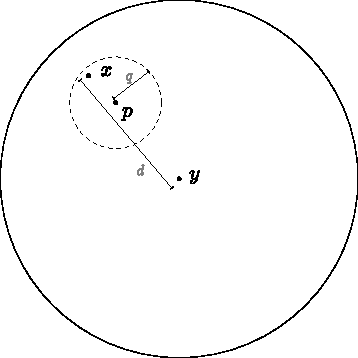
\includegraphics[scale=1]{fig/ball.pdf}
\end{figure}


Since we have shown both inclusions, it follows that the topology generated by $\mathcal{C}$ is the same as the standard topology on $\mathbb{R}^n$.


\begin{exer}[5 points]
	Let $T$ be the collection of subsets of $\mathbb{R}$ consisting of $\emptyset$ and every set $U$ such that $\mathbb{R} \setminus U$ is finite. Show that $T$ is a topology for $\mathbb{R}$. If $T_S$ is the standard topology for $\mathbb{R}$, is $T = T_S$, $T \subseteq T_S$ or $T_S \subseteq T$?
\end{exer}
{\color{blue}Collaborators: None.}

\textbf{$T$ is a topology:} To show that $T$ is a topology on $\mathbb{R}$, we must show that it contains $\varnothing$ and $\mathbb{R}$ and is closed under arbitrary unions and finite intersections.

\begin{enumerate}
	\item By definition, $T$ contains $\varnothing$. Then $\mathbb{R}-\mathbb{R}=\varnothing$, which is finite, so $\mathbb{R} \in T$.
	\item Consider the arbitrary union $\bigcup_{\alpha}U_\alpha$ of elements of $T$. Its complement $\mathbb{R}-\bigcup_{\alpha}U_\alpha$ is equivalent to, by DeMorgan's Laws, $\bigcap_{\alpha}(\mathbb{R}-U_{\alpha})$. Each of the $(\mathbb{R}-U_{\alpha})$ is finite by assumption, so their intersection must also be finite. Thus $T$ is closed under arbitrary unions.
	\item Consider the finite intersection $\bigcap_{i=1}^N U_i$ of elements of $T$. Then again by DeMorgan's Laws, $\mathbb{R}-\bigcap_{i=1}^N U_i=\bigcup_{i=1}^N (\mathbb{R}-U_i)$. Each $(\mathbb{R}-U_i)$ is finite, and the finite union of finite sets is itself finite. Thus $T$ is closed under finite intersections.
\end{enumerate}
\textbf{$T$ is strictly coarser than $T_S$:} We claim that $T$ is a proper subset of $T_S$. Any element of $T$ has a complement of the form $\{x_i\}_{i=1}^N$, so any element of $T$ is of the form $\mathbb{R}-\left\{ x_i \right\}_{i=1}^N$. If we order the $x_i$ in increasing order, this coincides with the set
\[
	(-\infty, x_1) \cup (x_1, x_2) \cup \cdots \cup (x_{N-1},x_N) \cup (x_N, \infty),
\] which is open in $T_S$ since it is the union of open intervals of $\mathbb{R}$. Thus $T \subset T_S$.

This is in fact a strict inequality. Take arbitrary $a < b$, then the interval $(a,b)$ is open in $\mathbb{R}$, yet its complement is $\mathbb{R}-(a,b) = (-\infty,a] \cup [b,\infty)$ is infinite. Thus $(a,b)$ is in $T_S$ but not in $T$, so $T$ is a strict subset of $T_S$.

\begin{exer}[5 points]
	Let $C$ denote the unit circle $\{(x, y)\ |\ x^2 + y^2=1 \}$ in $\mathbb{R}^2$ and let $[0, 1)$ denote the half-open interval $\{t\ |\ 0 \leq t < 1 \}$ in $\mathbb{R}$. Endow $C$ and $[0, 1)$ with the subspace topology from $\mathbb{R}^2$ and $\mathbb{R}$, respectively. Define $f: [0, 1) \to C$ by $f(t) = (\cos(2\pi t), \sin(2\pi t))$. Is $f$ a homeomorphism?
\end{exer}
{\color{blue}Collaborators: None.}

The map $f$ is \textit{not} a homeomorphism, as its inverse is not continuous. We demonstrate this by finding an open set $U$ in $[0, 1)$ such that $(f^{-1})^{-1}(U) = f(U)$ is not open in $C$.

Let $U = [0, 1/2)$. This is open in $[0, 1)$, as it is the intersection of $[0,1)$ and an open set, say $(-1, 1/2)$, of $\mathbb{R}$. Then $f(U)$ is the upper half of the unit circle, including the point $(1, 0)$ and excluding the point $(-1, 0)$. This is \textit{not} open in $C$, though, since for any $\varepsilon > 0$, the ball $B( (1,0), \varepsilon)$ intersected with $C$ is not entirely contained in $C$.

\end{document}
